This section gives a detailed view of the physical and logical infrastructure.

\subsubsection{High level component}
The app has been designed by applying the three layers architecture; this pattern, also kown as the n-tier architecture, is the de facto standard for most Java EE applications and devide in a well defined way the application's parts  by assigning a specific role to each layer.
\begin{itemize}
	\item \textbf{Presentation Layer:} It is the front end layer, it consists in the external interfaces and it is composed by three 			sublayers: two mobile application  dedicated to mobile devices, one for users and one for third parties, and a web browser for 			third parties.\\ Both mobile apps  includes only the presentation login and all sublayers directely interface with the app layer.
	\item \textbf{Application Layer:} It encases the app's core capability, this means that containts the whole logic included the main 		algorithms. 
	\item \textbf{Data Layer:} It includes the data storage system and data access. Data are accessed by the application layer 			via API call.
\end{itemize}In the following Figure the external services have been included to underline the fact that they interface with both presentation and application tier and it also underlines the fact that layers are closed. A closed layer means that a request moves from layer to layer and it  must pass through all layers right below before reaching the destination one.

\begin{figure}[h!]
	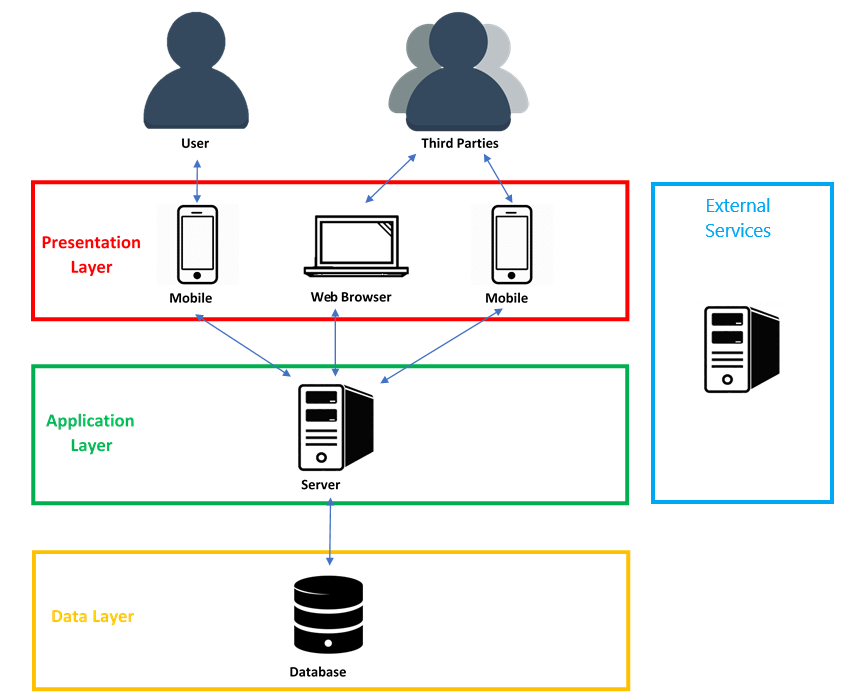
\includegraphics[width=1.0\textwidth]{./pictures/design_arch.png}\par
	\caption{Three-tiers architecture}
\end{figure}
\FloatBarrier

The next diagram shows interactions between all main components of the system. Because of the presence of two different stakeholders with different needs the client has been splitted in two according to the division in 2 different apps explained in the RASD. Althought this client's division the server has been maintained unique to avoid possible code redundancy and because most of the logic is related to the Third Party's app.

\begin{figure}[h!]
	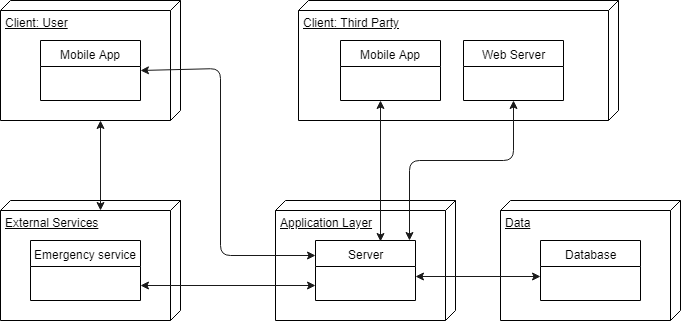
\includegraphics[width=1.0\textwidth]{./pictures/high_level_diagram.png}\par
	\caption{High Level Components}
\end{figure}
\FloatBarrier